\section{Theoretical Background} \label{sec:Theoretical}

This section presents the main concepts, which provide subsidies for the proposed project development.

%\subsubsubsection

%\input{chapters/2_THEORETICAL_BACKGROUND/sections/1_blockchain.tex}
%\input{chapters/2_THEORETICAL_BACKGROUND/sections/2_fundamentalsOfBlockchain.tex}
%\input{chapters/2_THEORETICAL_BACKGROUND/sections/4_smartContracts.tex} 
%\input{chapters/2_THEORETICAL_BACKGROUND/sections/5_traceability.tex}

%%%%%%%%%%%%%%%%%%%%%%%%%%%%%%%%%%%%%%%%%%%%%%
\subsection{Blockchain}\label{sec:blockchain}
Recently, cryptocurrency has attracted extensive attention from both industry and the academy. Bitcoin, which is often called the first cryptocurrency, had a huge success with the capital market coming to \$ 10 billion in 2016 \cite{coindesk}. Blockchain is the central mechanism of the Bitcoin and was first proposed in 2008 and implemented in 2009 \cite{nakamoto2008bitcoin}. The blockchain can be considered as a public ledger, in which All committed transactions are stored in a block chain. This chain grows continuously when new blocks are attached to it \cite{zheng2016blockchain}.

While the system of financial institutions that serve as third parties reliable processors for processing payments work well for most still suffers from the shortcomings inherent in the model based on confidence. In addition, the cost of mediation increases transaction costs, which limits the practical minimum size of the transaction and eliminates the possibility of small occasional transactions. To solve these problems, \cite{nakamoto2008bitcoin} defined an electronic payment system called Bitcoin, based on cryptographic proof rather than reliable, allowing either party willing to transact directly with each other without the need to a reliable third party.

This revolution began with a new marginal economy on the Internet. Bitcoin emerges as an alternative currency issued and not backed by a central authority, but by automated consensus among networked users \cite{swan2015blockchain}.

For \cite{swan2015blockchain}, besides the currency ( "Blockchain 1.0"), smart contracts ("2.0") demonstrate how the blockchain is in a position to become the fifth disruptive computing paradigm after mainframes, PCs, Internet and mobile/ social networks. Bitcoin is starting to become a digital currency, but technology blockchain behind it can be much more significant.

Potential benefits of blockchain are more than just economic. They extend to the political, humanitarian, social and scientific domains. Its technological capacity is already being harnessed by specific groups to solve real world problems.

\subsection{Fundamentals of blockchain}\label{sec:fundamentals}

Blockchain technology has key features such as centralization, persistence, anonymity and auditability. Blockchain can function in a decentralized environment that is activated by the integration of several key technologies such as cryptographic hash, digital signature and distributed consensus engine. As a transaction may occur in a decentralized manner, blockchain can greatly save the cost and improve efficiency \cite{zheng2016blockchain}. The main properties of the blockchain are considered innovative and enable rapid adoption for technology \cite{greve2018blockchain}:

\begin{itemize}
\item Decentralization;
\item Availability and integrity;
\item Transparency and auditability;
\item Immutability and Irrefutability;
\item Privacy and Anonymity;
\item Disintermediation;
\item Cooperation and Incentives.
\end{itemize}

%%%%%%%%%%%%%%%%%%%%%%%%%%%%%%%%%%%%%%%%%%%%%%

\subsubsection{Cryptography}\label{sec:criptografia}
Blockchain relies heavily on encryption to satisfy system and application security requirements. As the word suggests, cryptocurrencies also make heavy use of encryption. Encryption provides a mechanism for safely encoding the rules of a system encryption on the system itself. This can be used to prevent tampering and misconceptions. So, before be able to understand blockchains correctly, it is necessary to understand the cryptographic foundations \cite{narayanan2016bitcoin}. Cryptography is a deep academic field of research that uses many advanced mathematical techniques that are notoriously subtle and complicated \cite{narayanan2016bitcoin}.

\subsubsubsection{Cryptographic Hashes}\label{sec:hashesCriptograficos}
Hash is a mathematical function with the three properties to be follow \cite{narayanan2016bitcoin}:

\begin{itemize}
\item  Its input can be any string of any length;
\item Produces a fixed size output (eg., 256 digits);
\item It is efficiently computable. Intuitively, this means that for
a given input string, is possible to find out what is the hash function output within a reasonable period of time. Technically, hashing a n-bit string must have a $O(n)$ runtime.
\end{itemize}

These properties define a general hash function. Cryptographic hash functions (or cryptographic summaries) are unidirectional and hardly allow retrieving the original value $x$ from the hash $h$. For a hash function to be cryptographically safe, it must satisfy the following three properties: (1) collision resistance, (2) hiding and (3) puzzle friendliness \cite{greve2018blockchain}.

A collision occurs when two distinct inputs produce the same output. A hash function $H$ is collision resistant when it is impossible to find two values $x$ and $y$ such that $x \neq y$ and $H(x) = H(y)$ \cite{narayanan2016bitcoin}.

The hide property states that, having the hash function output $y = H (x)$, there is no possible way to find out which was the $x$ input \cite{greve2018blockchain}.

A hash function $H$ is considered puzzle friendliness if for each possible output value of $n$ bits $y$ if $k$ is chosen from a distribution with high min-entropy, then it is impracticable to find $x$ such that $H (k \| x) = y$ in time significantly less than $2^n$ \cite{narayanan2016bitcoin}.

\subsubsubsection{Digital Signatures}\label{sec:assinaturasDigitais}
A digital signature is supposed to be a digital analog of a handwritten paper signature. Two signature properties are desired which correspond well to the analogy of the handwritten signature: first, only one person can make their own signature, but anyone can verify if it is valid. Secondly, it is desired that the signature must be linked to a specific document, so the signature cannot be used to indicate the agreement or endorsement to a different document \cite{merkle1989certified}. Moreover, it is not possible to forge a signature in such a way as to reuse it in some other context. That is, signatures must be irrefutable.

To implement digital signatures, asymmetric key encryption is used. A secret key (sk) is used for signing the document and a public key (pk) is used to attest the signature's authenticity \cite{greve2018blockchain}.

A digital signature consists of the following algorithms \cite{narayanan2016bitcoin}:

\begin{itemize}
\item $(sk , pk) := generateKeys(keysize)$ – The $generateKeys()$ method receives a key size $(keysize)$ in the input and return a pair of public $(pk)$ and private $(sk)$ keys.
\item $sig := sign(sk , msg)$ – The method $sign()$ receives a message $msg$ and a secret key $(sk)$ on entry and returns the signature $sig$ f that message under $sk$.
\item $isValid := veri f y(pk , msg , sig)$ – The method $verify$ receives a public key $(pk)$, a message $msg$ and a signature $(sig)$ as input, and returns a boolean value: $isValid = true$ if $sig$ is a signature valid for $msg$ under $pk$; $isValid = false$, otherwise.
\end{itemize}

The following two properties must be maintained:

\begin{itemize}
\item Authenticity: Signatures can be validated: \\ $verify(pk, message, sign(sk, message)) = = true$.
\item Signatures are existentially unfalsifiable: signature cannot be forged.
\end{itemize}

It is noted that \textit{generateKeys()} and \textit{sign()} can be random algorithms. In fact, generating keys should be randomized, because it should be generating different keys for different people. On the other hand, \textit{verify()} will always be deterministic \cite{greve2018blockchain}.

\subsubsection{Consensus}\label{sec:consenso}
The key to blockchain operation is that the network must agree collectively on the ledger's content. Instead of a central entity maintain control over information (such as a bank for example), the data is shared among all. This requires the network to maintain the consensus around the information recorded in the block chain. How this consensus is reached, affects the security and economic parameters of the protocol \cite{kostarev2017review}.

In this context, consensus emerges as a fundamental problem, since it allow distributed participants to coordinate their actions in order to reach common decisions, thereby ensuring the consistency of safety and system progress (liveness) \cite{greve2018blockchain}.

Reaching consensus in such an environment is a challenge. This is also a challenge for blockchain, because its network is distributed and there is no central node that ensures that ledgers on distributed nodes be all the same. Nodes do not need to trust other nodes. Thus, some protocols are required to ensure that ledgers on different nodes are consistent \cite{kostarev2017review}.

A good consensus algorithm means efficiency, security and convenience. Current common consensus algorithms still have many shortcomings. New consensus algorithms are created to solve some blockchain-specific problems \cite{zheng2016blockchain}.

\subsubsection{Distributed Ledger}\label{sec:livro}
Distributed ledger is a data structure distributed by several nodes or computing devices. Each node replicates and saves a identical ledger copy. Each participating node in the network updates independently \cite{greve2018blockchain}.

\subsubsubsection{Transactions}\label{sec:transac}
Blockchain is a public digital book that records online transactions. In it, transactions are recorded in a block without the help of third parties, such as a bank or payment processor. The blockchain algorithm automatically graphs and authenticates the transaction, which is immediately visible to all users, minimizing the possibility of fraud \cite{Bankrate2018}.

From a technical standpoint, the most fundamental definition of a transaction is an atomic event allowed by the underlying protocol. A transaction determines a sequence of state operations. It adds a transfer of asset or, generally speaking, a smart contract. In a basic case, the transaction girds a digital signature of the issuer holding the asset and the receiver's address, as well as inputs and outputs for transaction. Each transaction must contain both Inputs and Outputs just like in a accounting book. Entries indicate the previous transaction hash which is related to the current one \cite{greve2018blockchain}. Validating a Transition involves:

\begin{enumerate}
	\item signature verification;
	\item confirmation of existing values from hashes of previous referenced transactions;
	\item confirmation that the amount was not previously spent by any other transactions.
\end{enumerate}

\subsubsubsection{blocks}\label{sec:blocks}
Blocks contains a header with information needed for current maintenance and its validation. A block consists of the block header and block body as shown in Figure \ref{fig:block}. 
{\color{red} RETIRAR ESSA IMAGEM SE FOR PRECISO}
\begin{figure}[htbp]
\begin{center}
  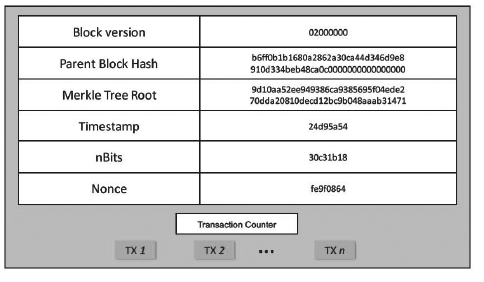
\includegraphics[scale=0.5]{images/blockStructure.png}
\caption{Structure of a block. \cite{zheng2016blockchain}}
\label{fig:block}
\end{center}
\end{figure}

The body's block consists of a transaction counter and transaction. The maximum number of transactions a block can hold depends on block size and the size of each transaction \cite{zheng2016blockchain}.

The validation of a block consists in verifying (i) if its structure is well formed (ii) its hash is valid (meets the challenge), (iii) its size is within the network accepted limit, (iv) the set of transactions within the block is valid, (v) the first transaction (and only the first) is the coinbase transaction - which incorporates the generation of new cryptocurrencies in the system, besides acting as a reward mechanism. The blocks are validated independently, by each node of the blockchain network, and this feature contributes to the process decentralization \cite{greve2018blockchain}.

%%%%%%%%%%%%%%%%%%%%%%%%%%%%%%%%%%%%%%%%%%%%%%
\subsubsection{Smart Contracts}\label{sec:smartContracts}

Blockchain 2.0 begins with the innovative proposal of smart contracts in 2013, and all range of possible financial applications \cite{greve2018blockchain}. A smart contract is a computerized transaction protocol that executes the terms of a contract \cite{szabo1997idea}. Its model was proposed a long time ago and now this concept can be implemented with blockchain.

The term smart contract (SC) has been standardized by Nick Szabo in the 90s \cite{greve2018blockchain}. It means: “an internal transaction protocol format that executes the terms of a contract. Their overall goals are ensure common contractual conditions (such as payment terms, liens, confidentiality and even compliance), minimize malicious and accidental exceptions and the need for reliable intermediaries. Related economic objectives include reducing fraud losses, arbitration and execution costs, and other transaction costs.” \cite{szabo1997idea}.

Smart contract searches can be classified into two types: development and evaluation. Development can be development of smart contract or smart contract platform development. Recently, many smart contracts have been implemented on the Ethereum blockchain \cite{wood2018secure}. Regarding the platform development, many smart contracting platforms like Ethereum \cite{wood2018secure} and Hawk \cite{kosbaa2016theblockchain} are emerging \cite{zheng2016blockchain}. Evaluation means code analysis and performance evaluation. Errors in smart contracting can bring disastrous damage. Smart contract attack analysis is very important. On the other hand, smart contract performance is also vital to the contract. With the rapid development of blockchain technology, more and more smart contract based applications will be placed in use and companies need to consider performance of application \cite{zheng2016blockchain}.

In the blockchain, smart contracts are created as scripts, stored in with exclusive addressing on the blockchain itself \cite{greve2018blockchain}. They are triggered when addressing a transaction to it. Then the script is executed independently and automatically, as prescribed in all nodes in the network according to the data included in the transaction \cite{christidis2016blockchains}.

\subsubsubsection{Smart Contracts Security}\label{sec:seguranca}
Smart contracts interpret the code objectively - "The Code is the law". However, a code error was the target of cyber attack, resulting in a deviation of about \$50 million dollars, forcing Ethereum to perform a hard fork to perform a recovery \cite{bashir2018mastering}. Performing recoveries like this is not trivial, so the risks must be evaluated and minimized.

Smart contracts should be concerned with blockchain threats:
\begin{itemize}
\item State of contract.
\item Random generation.
\item Time Restrictions.
\end{itemize}

Regarding the status of the contract, field and balance values determines the smart contract state. A user when invoking it may not have certainty under its state, as other transactions may modify it or a fork may have occurred. In some cases, this can create vulnerabilities and lead to asset theft. In random generation, some contracts generate pseudo-random numbers with the same seed for all miners. This allows everyone to have the same view as Blockchain, providing
a malicious miner to influence the network. About time restriction, if a miner holds a stake in a contract, he can gain an advantage by choosing an appropriate time stamp for the block he is exploring \cite{greve2018blockchain}.

%%%%%%%%%%%%%%%%%%%%%%%%%%%%%%%%%%%%%%%%%%%%%%

\subsection{Traceability}\label{sec:traceability}

There are billions of products being manufactured every day through complex supply chains that can extend to all parts of the world. However, there is very little information on how, when and where these products originated, manufactured and used during their life cycle \cite{horiuchirastreabilidade}.

Before reaching the end consumer, the goods go through an often wide network of retailers, distributors, carriers, warehousing facilities and suppliers who participate in the design, production, delivery and sales process of a product, but in many cases. These steps are a dimension invisible to the consumer \cite{provenance2015}.

In \cite{gryna1998juran, Opara2001} Traceability is defined as the ability to preserve the identity of the products and their origins, so that the collection, documentation and maintenance of information related to all processes in the production chain must be ensured. For a food product, traceability represents the ability to identify where and how it was grown, as well as the ability to track its post-harvest history and to identify the processes performed at each step in the production chain through records. Traceability is required primarily for \cite{horiuchirastreabilidade}:
\begin{itemize}
\item Improve credibility with customers and consumers.
\item Ensure that only quality materials and components are present in the final product.
\item Better allocate responsibilities.
\item Identify products that are distinct but may be confused.
\item Enable the return of defective or suspect products.
\item Find the causes of failures and take steps to repair them at the lowest possible cost.
\end{itemize}

In \cite{opara2003traceability} six important elements are to be considered for traceability:

\begin{itemize}
\item Product Traceability: Determines the location of a product at any stage of the production chain. to facilitate logistics, inventory management, product recall, and information disclosure to consumers and customers.
\item Process Traceability: Identifies the type and sequence of activities that affected a particular product. This includes any interactions between the product and physical / mechanical, chemical and environmental factors that result in the transformation of raw material into value added products.
\item Genetic Traceability: determines the genetic constitution of the product.
\item Input Traceability: Determines the type and source of input such as fertilizers and livestock.
\item Traceability of Diseases and Pests: Tracks the epidemiology of pests such as bacteria and viruses.
\item Measurement Traceability: determines the measurement instruments, in addition to specifying the environmental, geospatial and temporal factors that influence data quality.
\end{itemize}

A traceability system allows any user to track products by providing information about them (eg originality, components, or locations) during production and distribution. Suppliers and retailers typically require independent, government-certified traceability service providers to inspect products throughout the supply chain. Vendors and retailers request traceability services for different purposes.Suppliers want to receive certificates to showcase their products. Retailers want to verify the origin and quality of products \cite{lu2017adaptable}.

Supply chain visibility, or traceability, is one of the key challenges encountered in the business world, with most companies having little or no information about their own second- and third-tier suppliers. Transparency and end-to-end visibility of the supply chain can help shape product, raw material, test control, and end product flow, enabling better operations and risk analysis to ensure better chain productivity \cite{abeyratne2016blockchain}.

Folinas et al. \cite{folinas2006traceability} identified that the efficiency of a traceability system depends on the ability to track and trace each individual asset and logistics units, in a way that enables continuous monitoring from firstly processed until final clearance by the consumer.

Aung and Chang \cite{aung2014traceability} and Golan \cite{golan2004traceability} set three main traceability objectives, namely: (1) better supply chain management, (2) product differentiation and quality assurance, and (3) better identification of non-compliant products. An additional objective is to maintain assurance of traceability in accordance with applicable regulations and standards. A complete traceability system will include components that manage \cite{vargas2017trazabilidad}:

\begin{enumerate}
\item Identification, marking and assignment of traceable objects, parties and locations.
\item Automatic capture (by scanning or reading) of movements or events involving an object.
\item Record and share traceability data, internally or with parts of a supply chain, so that visibility of what has occurred can be achieved.
\end{enumerate}